	La littérature sur le sujet des ordonnanceurs est assez vaste. 
	Ceux-ci sont composés principalement de trois grandes familles :\medskip
	\begin{itemize}
		\item Les mono-processeurs
		\item Les multi-processeurs Partitionnés
		\item Les multi-processeurs Globaux
	\end{itemize}
	Les ordonnanceurs mono-processeurs étant plus simples à appréhender, nous commencerons 
	par présenter cette famille.
	
	\section{Ordonnanceurs mono-processeur}
	\subsection{Ordonnanceurs à priorité fixe sur tâche}
	
	\subsubsection{Rate Monotonic}
	L'ordonnanceur \customhighlight{R}ate \customhighlight{M}onotonic (RM) est décrit par Liu et Layland \cite{liu_scheduling_1973} en 1973. C'est 
	donc un ordonnanceur classique, bien connu, ainsi que largement documenté \cite{kermia_ordonnancement_2009}. 
	L'idée de base est qu'une tâche avec une période courte évolue rapidement, et 
	doit donc être prioritaire.\medskip
	On considère un ensemble de tâches périodiques et indépendantes.
	Les priorités sont statiques et attribuées en fonction de la durée de la période, ainsi 
	la tâche avec la période la plus faible sera de priorité plus élevée. 
	Un des points fondamentaux de l'article est la preuve de l'optimalité de RM dans le cas 
	préemptif, à tâches périodiques, à échéance sur requête, indépendantes, simultanées.
	Les auteurs énoncent même une condition suffisante d'ordonnançabilité pour un système à $m$ tâches : \medskip
	\begin{center}
		$\sum_{i=1}^{m}\frac{C_i}{T_i} \leq m(2^{\frac{1}{m}}-1)$
	\end{center}
	Notons également que pour $m \rightarrow \infty$, $\sum_{i=1}^{m}\frac{C_i}{T_i} \leq m(2^{\frac{1}{m}}-1) \rightarrow \ln(2) \approx 0.69$.
	Une condition suffisante est donc que le facteur d'utilisation du système soit inférieur à 0.69. 
	Dans ce cas, le système est ordonnançable par RM.\medskip
	
	Des améliorations ont par la suite été apportées par Joseph et Pandya \cite{joseph_finding_1986},
	qui ont trouvé une condition nécessaire et suffisante. 
	Ainsi, si $RT(t_i)$ est le temps de réponse (\ref{Response Time}) d'une tâche $t_i$, 
	alors si un ensemble de tâches périodiques est trié par ordre décroissant, l'équation 
	récurrente suivante 
	définit la borne supérieure du temps de réalisation, lorsqu'elle tend vers un point fixe :
	\begin{center}
		$RT(t_i)^{q+1} = \sum_{j=1}^{i-1} \lceil \frac{RT(t_i)^q}{T(t_i)} \rceil \times C(t_j) + C(t_i)$
	\end{center}
	Le système est ordonnançable si et seulement si $\forall i_{(1 \leq i \leq m)}$, $RT(t_i) \leq D_i$.
	On pourra résoudre récursivement cette équation afin de prouver son ordonnançabilité.\medskip
	
	\textit{RM} n'est cependant optimal que pour cette classe de tâches. Dès que les propriétés changent, 
	il faudra se tourner vers un autre type d'ordonnanceur.
	
	
	\subsubsection{Deadline Monotonic}
	Deadline Monotonic (DM) est un ordonnanceur optimal pour la classe de systèmes à départ 
	simultanés et à échéances contraintes. 
	Il a été décrit par Leung et Whitehead 
	\cite{leung_complexity_1982}. Cet article aborde le point de vue mono-processeur et multi-processeur partitionné, 
	dont il sera question plus loin dans ce document.\medskip
	
	Avec cet ordonnanceur, les priorités sont fixes, au niveau des tâches.
	Plus l'échéance est petite, plus la priorité est élevée. On peut considérer que \textit{RM} est 
	un cas particulier de \textit{DM}, puisque pour \textit{RM}, les tâches sont à échéance sur requête \ref{echeancesurrequete}.
	Il n'existe pas de test d'ordonnançabilité basé sur l'utilisation du système. Pour vérifier celle-ci, 
	il faut avoir recours à l'équation décrite plus haut. 
	On peut la résoudre itérativement à l'aide de ce système d'équations: \medskip
	\begin{enumerate}
		\item $W_0 = C_i $
		\item $W_{k+1} = C_i + \sum_{j = 1}^{i-1}\lceil \frac{W_k}{T_j} \rceil \times C_j $
	\end{enumerate}
	
	
	\subsection{Ordonnanceurs à priorité fixe sur travail}
	\subsection{Earliest Deadline First}
	\customhighlight{E}arliest \customhighlight{D}eadline \customhighlight{F}irst (EDF) est un ordonnanceur 
	qui a été introduit en 1973, dans le même article que celui où est présenté Rate Monotonic 
	par Lui et Layland \cite{liu_scheduling_1973}. 
	C'est un ordonnanceur capable d'ordonnancer aussi bien les tâches à départs simultanés que celles 
	à départs différés, et les tâches à échéances contraintes ainsi 
	qu'arbitraires (pas de contrainte sur l'échéance par rapport à la période). 
	Il fixe les priorités sur les travaux. L'assignation de la priorité se fait sur base de 
	la proximité de l'échéance absolue : Plus cette échéance est proche et plus la priorité est élevée. 
	Une façon déterministe et arbitraire de régler les cas d'égalité doit être décidée.\medskip
	
	\textit{EDF} est optimal pour toutes les tâches synchrones et asynchrones, avec et sans 
	contraintes sur les échéances. 
	Cela signifie que si un système est ordonnançable, \textit{EDF} peut l'ordonnancer.\medskip
	Cette propriété est importante, car les classes de tâches ordonnancées par \textit{EDF} 
	sont plus larges que \textit{RM} et \textit{DM}, par conséquent, \textit{EDF} peut ordonnancer également les 
	mêmes classes qu'\textit{RM} et \textit{DM} en conservant son optimalité. \medskip
	
	Les tests de faisabilité avec \textit{EDF} dépendent de la classe de tâche considérée. 
	Pour un système synchrone et à échéance sur requête, 
	une condition nécessaire et suffisante de faisabilité est donc que l'utilisation soit inférieure 
	à 100\%, c'est-à-dire : \medskip
	\begin{center}
		$\forall \tau_i \in \Gamma_m, \sum_{i=1}^{m}\frac{C_i}{T_i} \leq 1 $
	\end{center}
	
	Dans le cas d'un système synchrone à échéance arbitraire, l'intervalle de temps qu'il est 
	nécessaire de vérifier est $[0, L]$ avec $L$ qui peut se calculer de façon itérative en cherchant un point fixe 
	avec cette formule : \medskip
	\[
	\left \{
	\begin{array}{r l}
	W_0 &= \sum_{i = 1}^{m}C_i\\
	W_{k+1} & =\sum_{i = 1}^{m} \lceil \frac{W_k}{T_i} \rceil \times C_i
	\end{array}
	\right.
	\]
	
	Dans le cas des systèmes de tâches asynchrones, l'intervalle considéré est plus grand : 
	$[0, O_{max} + 2 \times P]$ avec $O_{max}$ l'offset maximum du système et 
	$P$ le plus petit commun multiple ($ppcm$) de toutes les périodes du système, soit : \medskip
	\begin{center}
		$P = ppcm\{T_i | i \in \{1, ... m\}\}$
	\end{center}
	
	Malgré le fait que la littérature montre la supériorité d'\textit{EDF} sur \textit{RM}, 
	il semble que ce soit RM qui soit plus volontiers choisi pour implémentation. 
	Sa réputation est qu'il est plus simple. 
	On trouve un résumé du débat qui existe à ce sujet dans un article de Buzzato~
	\cite{buttazzo_rate_2005}.
	
	\section{Multi-processeurs : les différentes familles d'ordonnanceurs}
	
	Dans la partie précédente, nous avons présenté certains algorithmes mono-processeur, 
	ainsi que quelques conditions d'ordonnançabilité.
	De nos jours, une grande partie des architectures employées dans les systèmes embarqués 
	est multi-processeur. 
	Les stratégies mises en place pour l'ordonnancement de tels 
	systèmes sont différentes. Dans la littérature, il est habituel de présenter 
	deux familles principales d'ordonnanceurs multi-processeurs :\medskip
	\begin{itemize}
		\item Les ordonnanceurs partitionnés
		\item Les ordonnanceurs globaux
	\end{itemize}
	Nous verrons qu'une troisième famille est souvent présentée également. Elle représente un 
	mélange des deux précédentes. On parle d'ordonnanceurs \textit{hybrides}, ou \textit{semi-globaux}.
	
	\section{Les ordonnanceurs partitionnés}
	L'idée principale derrière la stratégie du partitionnement est que pour tout 
	ensemble $\Gamma$ de $n$ tâches, si l'utilisation de chaque tâche est inférieure à $1$ 
	($\forall i \in \{1, n\}, U_i < 1$), soit $m$ le nombre de processeurs,  
	alors il existe un ordonnanceur de $m \leq n$ processeurs capable d'ordonnancer cet ensemble. 
	Il y a principalement deux optiques différentes pour envisager ce problème : \medskip
	\begin{itemize}
		\item Partir de l'ensemble maximum et appliquer un algorithme de recherche afin de trouver 
		la valeur de $m$ la plus petite telle que l'ordonnancement soit possible
		\item Résoudre ce problème connu dans la littérature comme celui du \customhighlight{Bin-Packing}, 
		et rejoindre un domaine bien connu et largement documenté.
	\end{itemize}
	Dans la suite du document, on ne s'intéressera qu'aux heuristiques liées au \customhighlight{Bin-Packing} et 
	laisserons de côté les algorithmes de recherche.
	
	\subsection{Ordonnanceurs à priorité fixe sur tâche}
	
	La stratégie de partitionnement consiste à diviser l'ensemble de tâches en sous-ensembles qui seront 
	attribués à un processeur particulier. Cela permet de conserver les mêmes algorithmes ainsi 
	que tests d'ordonnançabilité que ceux 
	décrits précédemment puisqu'en divisant le système en sous-systèmes attribués à un 
	processeur chacun, cela revient à appliquer \og localement\fg{}  une stratégie mono-processeur, contre 
	une stratégie globale multi-processeur \cite{ndoye_ordonnancement_2014}.
	
	Concrètement, cela revient à diviser un ensemble $\Gamma$ de tâches en $n$ sous-ensembles 
	$\gamma \in \Gamma$ et d'attribuer à chacun des $m$ processeurs un de ces sous-ensembles $\gamma$.\medskip
	
	
	Le problème du partitionnement consiste donc en premier lieu 
	à résoudre une division du système en sous-systèmes, ce qui est connu dans la 
	littérature scientifique comme le problème du bin-packing \cite{ausiello_approximation_1984}.
	Ce problème est $NP$ difficile, si bien qu'en pratique, 
	des heuristiques sont appliquées, comme par exemple :\medskip
	\begin{itemize}
		\item \textit{First-fit} 
		\item \textit{Best-fit}
		\item \textit{Next-fit}
	\end{itemize}
	
	Plusieurs algorithmes de ce type ont été présentés dans la littérature scientifique
	dans les années 80 comme par exemple \cite{dhall_real-time_1978} dans ce 
	document de Dhall et Liu en 1978. 
	Dans leur article, ils donnent notamment des fourchettes d'utilisations 
	permettant d'ordonnancer pour le cas multi-processeur utilisant \textit{RM}, 
	considérant les échéances implicites :
	\begin{mytheorem}
		\textit{\og Si un ensemble de $m$ tâches est ordonnancé selon l'algorithme \textit{Rate-Monotonic}, 
			alors le facteur d'utilisation minimum réalisable est $m\times(2^{\frac{1}{m}} - 1)$\fg{} .}
	\end{mytheorem}

	Ils ajoutent :\medskip
	\textit{En déduction, si $m$ tend vers l'infini, alors l'utilisation minimale possible approche $ln(2)$.}
	
	Dans cet article, ils décrivent également :\medskip
	\begin{itemize}
		\item \textbf{RMNFS} : \textit{Rate Monotonic Next-Fit Scheduler}
		\item \textbf{RMFFS} : \textit{Rate Monotonic First-Fit Scheduler}
	\end{itemize}
	\vspace{1em}
	qui finalement, sont des algorithmes basés sur \textit{RM} dont le système de tâche est 
	réparti selon les algorithmes heuristiques de \textit{bin-packing} \textit{Next-Fit} et \textit{First-Fit}. 
	Afin de trier les tâches, on considère leur utilisation.
	
	Par la suite, d'autres algorithmes basés sur \textit{RM} et \textit{DM} avec 
	heuristique de bin-packing sont proposés et leurs performances analysées. 
	Un historique complet est proposé dans le travail de thèse de Ndoye \cite{ndoye_ordonnancement_2014}. 
	Les recherches tendent à trouver des conditions d'ordonnançabilité utiles.\medskip
	
	Ce pan des ordonnanceurs est donc très bien connu à ce jour, très bien documenté. 
	Dans ces conditions, il n'est pas étonnant de voir que ces solutions sont encore largement 
	répandues dans l'industrie à ce jour, les algorithmes \textit{RM} et \textit{DM} 
	étant assez simples à implémenter, des heuristiques ainsi que leur efficacité ayant été analysées, en théorie ainsi qu'en pratique.\medskip
	
	Un défaut majeur de ces algorithmes est que bien souvent, l'utilisation des processeurs sera 
	sous-performante, ce qui est une raison très souvent invoquée dans la littérature pour se 
	tourner vers d'autres solutions. 
	Andersson, Baruah et Jonsson proposent RM-US$\frac{m}{3m-2}$ avec un test 
	d'ordonnançabilité plus permissif \cite{andersson_static-priority_2001}. Ils prouvent 
	qu'un système est réalisable sous deux conditions :\medskip
	\begin{itemize}
		\item $\forall \tau_i \in \tau, U_i \leq \frac{m}{3m-2}$
		\item $U(\tau) \leq \frac{m^2}{3m-2}$ 
	\end{itemize}
	\vspace{1em}
	Pour arriver à ces conditions, l'algorithme d'attribution des priorités est légèrement modifié : \medskip
	\begin{itemize}
		\item si $U_i > \frac{m}{3m-2}$, $\tau_i$ a la plus grande priorité
		\item sinon, $\tau_i$ se voit assigner une priorité sous les mêmes conditions que \textit{RM}.
	\end{itemize}
	
	
	\subsection{EDF partitionné}
	Il a été rappelé plus tôt dans ce document qu'\textit{EDF} mono-processeur est optimal, 
	c'est-à-dire qu'il peut ordonnancer tout type de système qui est ordonnançable. 
	Malheureusement, ce résultat n'est pas valable dans le cas multi-processeur \cite{dertouzos_multiprocessor_1989}.\medskip
	
	Cet algorithme a lui aussi été adapté à une utilisation multi-processeur en y joignant 
	des heuristiques de bin-packing : \medskip
	Dans \cite{pereira_zapata_edf_2005}, Zapata et Alvarez décrivent les algorithmes 
	EDF avec partitionnement préalable, par exemple : \medskip
	\begin{itemize}
		\item EDF-FF (\textit{first-fit})
		\item EDF-NF (\textit{next-fit})
		\item EDF-WF (\textit{worst-fit})
		\item EDF-NFD (\textit{next fit decreasing})
	\end{itemize}
	et proposent une analyse de la complexité. Ils renvoient eux-mêmes vers 
	\cite{lopez_utilization_2004} 
	qui est cité de nombreuses fois et semble être la référence à propos de ces algorithmes. 
	Dans cet article, Lopez, Diaz et Garcia proposent une limite de l'utilisation à la 
	ordonnançabilité en fonction de l'algorithme d'attribution des tâches. Ces conditions 
	sont suffisantes, mais pas nécessaires.\medskip
		
	\subsection{Avantages et inconvénients des ordonnanceurs partitionnés}
	\subsubsection{Avantages}
	Nous avons vu dans les sections précédentes que les algorithmes d'ordonnanceurs 
	partitionnés sont bien documentés, et présentent un certain nombre d'avantages parmi lesquels 
	le fait d'être bien connus aussi bien en pratique qu'en théorie. 
	Certains algorithmes donnent même de bons résultats, et l'on pourrait se satisfaire de 
	cette famille d'algorithmes. De nouvelles études et améliorations sont encore à ce jour proposées 
	dans des recherches récentes \cite{rodriguez_paul_multi-criteria_2013}.\medskip
	
	\subsubsection{Inconvénients}
	Toutefois, ces algorithmes présentent quelques inconvénients. 
	L'un d'eux est que leur résolution ne garantit pas de trouver la solution optimale, 
	puisque ce sont des heuristiques. 
	Il n'est pas envisageable de penser 
	que ces algorithmes puissent donc être optimaux pour une famille de tâches.
	
	Un autre problème important est que dans le processus partitionné, une tâche est 
	assignée à un seul processeur. 
	Ainsi, si des solutions existent qui consistent à migrer une tâche sur un autre processeur, 
	elles ne pourront pas être trouvées 
	par un ordonnanceur partitionné \cite{ramamurthy_static-priority_2000}. 
	Enfin, une autre limite est que ce processus ne permet pas à une tâche d'évoluer avec le temps. 
	Ses propriétés doivent être fixes. 
	Cela peut convenir à un certain nombre de systèmes, mais ne peut pas être une solution générale.
	De façon générale, on retrouve dans la littérature l'idée que les ordonnanceurs globaux 
	permettent généralement d'ordonnancer plus de systèmes que les ordonnanceurs partitionnés, 
	mais la conclusion ne peut être considérée comme définitive : cela dépend des situations
	\cite{lopez_utilization_2004}.
	Il y a aussi un problème lié à la communication entre les tâches. Dans nos recherches, 
	la plupart des articles posent que les tâches sont indépendantes entre elles. Dans 
	la réalité, les tâches sont souvent dépendantes, elles doivent communiquer, ce qui pose 
	des problèmes de précédence. 
	L'approche partitionnée gère plusieurs ordonnanceurs indépendants entre eux, si bien 
	que chaque système pourra gérer ces communications localement, mais pas les systèmes entre eux. 
	\medskip
	
	Il est connu que les algorithmes d'ordonnanceurs globaux et partitionnés ne sont pas comparables, 
	pour la principale raison que les ordonnanceurs partitionnés ne permettent pas de faire des 
	\textit{migrations} [\ref{migration}]. Dans l'article \cite{baruah_techniques_2007}, \textit{Baruah} 
	compare les deux techniques pour des systèmes de tâches \textit{sporadiques}, et 
	ses recherches montrent plusieurs résultats importants :\medskip
	\begin{mylemme}
		il y a des systèmes de tâches ordonnançables avec des algorithmes globaux à priorité fixe 
		sur travail que des algorithmes partitionnés à priorité fixe sur travail ne peuvent pas ordonnancer.
	\end{mylemme}
	
	\begin{mylemme}
		il y a des systèmes de tâches ordonnançables avec des algorithmes partitionnés à priorité fixe 
		sur travail que des algorithmes globaux à priorité fixe sur travail ne peuvent pas ordonnancer
	\end{mylemme}
	Ceci est prouvé en détaillant des contre-exemples dans l'article et permet de conclure :\medskip
	\begin{mytheorem}
		Les ordonnanceurs globaux et partitionnés à priorités fixes sur travail sont incomparables.
	\end{mytheorem}
	Cela ne dit rien des autres classes, et ne peut pas être généralisé. C'est 
	un résultat cependant important, qui montre que le fait de permettre les migrations
	change considérablement le comportement des ordonnanceurs.
	
	\section{Ordonnanceurs multi-processeurs globaux}
	Un ordonnanceur global est un ordonnanceur qui gère un ensemble de processeurs et 
	un système de tâches. Il ne procède pas à un tri préalable comme dans le cas partitionné. 
	Il gère une \textit{queue} de $n$ tâches prêtes à être exécutées 
	qui peuvent être assignées à $m$ processeurs à chaque fois que l'ordonnanceur en a l'occasion.\medskip
	
	Les algorithmes mono-processeurs vus précédemment peuvent donc être adaptés 
	à ce type de stratégie facilement : en attribuant les priorités à toutes les tâches, et en 
	exécutant plusieurs travaux sur plusieurs processeurs. 
	Plusieurs résultats qui viennent assombrir les perspectives d'une adaptation aussi simple. \medskip
	
	\subsection{L'Effet Dhall}
	Dans leur article de 1978 \cite{dhall_real-time_1978}, Dhall et Liu montrent que certains ordonnanceurs 
	initialement mono-processeurs, (\textit{RM} ou \textit{EDF}) peuvent donner lieu à une utilisation faible des 
	processeurs, ce qui signifie qu'ils ne seraient pas utilisés de façon optimale.\medskip 
	Par ailleurs, il a été montré que pour certains algorithmes, 
	il existe des systèmes qui présentent des \textit{pathologies}.
	Cela signifie que certains systèmes ne sont pas ordonnançables malgré une 
	utilisation totale de $1 + \epsilon$ et ce quel que soit le nombre de processeurs $m$.
	La déduction suivante peut en être tirée : la limite de l'utilisation totale 
	pour RM ou EDF est de $1 + \epsilon$, avec $\epsilon$ arbitrairement petit, ce 
	quel que soit $m$. 
	
	Cela est connu dans la littérature comme l'\og effet Dhall\fg{}  (Dhall's effect) et remet en 
	question l'intérêt de baser les tests de ordonnançabilité sur l'utilisation totale, et 
	montre que d'autres facteurs devraient être pris en considération. Dans un premier temps, cependant, 
	cela a participé à montrer la supériorité des approches partitionnées, ce pourquoi elles ont 
	largement été plus étudiées dans les années 80-90 \cite{davis_survey_2011}.\medskip
	
	De plus, dans le cas global, les \ref{instantcritique}{instants critiques} ne sont plus aussi faciles à prédire 
	que dans le cas mono-processeur. \medskip
	
	\subsection{Anomalies}
	Les anomalies sont décrites dans la littérature comme des changements qui intuitivement ne devraient 
	pas affecter l'ordonnançabilité des tâches, et qui rendent cependant le système non-ordonnançable. 
	Cela peut se produire dans diverses circonstances, comme par exemple :\medskip
	\begin{itemize}
		\item le temps d'exécution décroît
		\item La période d'une tâche augmente
	\end{itemize}
	et le système qui était auparavant ordonnançable ne l'est plus.
	
	
	
	\subsection{Priorité fixe sur tâche : RM/DM global}
	Si l'assignation des priorités \textit{RM} (ou \textit{DM}) en version multi-processeur global 
	fonctionne de la même façon que dans sa version mono-processeur - 
	c'est-à-dire, la priorité la plus élevée est accordée à la tâche qui a la période la plus faible - 
	\textit{RM} est donc concerné par l'effet Dhall. \medskip
	
	
	\subsection{Priorité fixe sur travail : EDF}
	Comme pour \textit{RM} et \textit{DM}, \textit{EDF} peut simplement être adapté à une exécution multi-processeur, 
	considérant un ensemble $n$ de tâches sur $m$ processeurs. Mais le gros avantage d'\textit{EDF} 
	dans sa version mono-processeur est son optimalité, qui n'est malheureusement pas conservée ici. 
	Plusieurs versions globales reposant sur \textit{EDF} sont décrites dans la littérature. 
	Il y a \textit{EDF} appliquant \textit{First Fit Decreasing Utilization}, décrit par 
	Lopez et al. \cite{lopez_utilization_2004}, où l'on obtient ces conditions d'ordonnançabilité : \medskip
	$U(\tau) \leq \frac{(m + 1)}{2}$ et $U_{max} \leq 1$. \medskip
	Un autre exemple est EDF-US. 
	Dans ce cas, la priorité des tâches est assignée légèrement différemment :\medskip
	\begin{itemize}
		\item si $U_i > \frac{m}{2m-1}$, la tâche $\tau_i$ se voit assigner la plus haute priorité
		\item sinon on applique les mêmes règles que pour \textit{EDF} mono-processeur
	\end{itemize}
	Une condition suffisante est alors :\medskip
	$U = \sum_{i=1}^{n}\frac{C_i}{T_i} \leq \frac{m^2}{3m-2}$
	alors le système de tâches est ordonnançable sur $m$ processeurs
	\cite{andersson_static-priority_2001}. \medskip
	D'autres documents encore décrivent des conditions d'ordonnançabilité et sont régulièrement 
	cités comme références comme de nombreux articles de Baker 
	\cite{baker_multiprocessor_2003} \cite{baker_analysis_2005} ou Baruah \cite{baruah_optimal_2004}
	\cite{baruah_schedulability_2008}. 
	Dans cet article de Davis et Burns, les auteurs rappellent les 
	limites supérieures d'utilisation pour ces techniques \cite{davis_survey_2011}.\medskip
	
	
	\subsection{Il n'existe pas de stratégie en ligne optimale sans clairvoyance}
	Quelques résultats déjà connus dans la littérature montrent que le sujet est difficile. 
	En effet, dans leur article de 1988 \cite{hong_-line_1988}, Hong et Leung montrent :\medskip
	\textit{\og Pour tout $m > 1$, il n'existe pas d'ordonnanceur en ligne optimal pour les ensembles 
	de travaux avec au moins deux échéances distinctes\fg{}}. 
	Un autre article de Fisher et al \cite{fisher_optimal_2010} élargit cela aux tâches sporadiques. 
	Ces résultats, quoi que négatifs, ne peuvent être généralisés à toutes les classes de tâches. 
	
	C'est un résultat embarrassant, toutefois, de nombreuses publications ultérieures ont montré des algorithmes 
	optimaux pour d'autres classes de tâches. 
	Par ailleurs, ce résultat est juste dans le cas d'un ordonnanceur non-clairvoyant, 
	mais ne peut pas être généralisé dans le cas où 
	l'algorithme a accès à des données sur les tâches au préalable.
	
	\subsection{PFair}
	En 1996, Baruah et al. décrivent l'algorithme \textit{PFair}. \cite{baruah_proportionate_1996}
	L'article apporte plusieurs définitions importantes :
	
	
	Soit $x$, une tâche. 
	Posons que $x.w$ représente le \og poids\fg{} , défini de cette façon : 
	
	$x.w = \frac{x.e}{x.p}$ où
	$x.e$ représente le nombre d'unités de temps nécessaires à la réalisation de la tâche 
	$x$	et $x.p$ la période. Ainsi, $0 < x.w < 1$.
	
	\begin{mydef}
		$Lag(S, x, t) = x.w \times t - \sum_{i\in[0,t)}^{max} S(x, i)$, où 
		$S$ est un ordonnanceur, $x$, un travail, $t$ un instant, et où $S(x, t) = 1$ si 
		le travail $x$ est exécuté à l'instant $t$, $0$ sinon.
	\end{mydef}
	\begin{mydef}
		Un ordonnanceur est P-fair si et seulement si :
		
		
		$\forall x, t : x \in \Gamma, t\in , \mathbb{N} : -1 < lag(S,x,t) < 1$
	\end{mydef}
	\begin{mytheorem}
		La P-équité (PFairness) implique que toutes les échéances soient satisfaites.
	\end{mytheorem}
	
	PFair est associé dans la littérature à l'idée de \textit{P-Fairness}, qui est une notion 
	idéale permettant de prouver des propriétés importantes pour le domaine. 
	L'une d'elle est que chaque ordonnanceur P-Fair est périodique. \medskip
	
	Il s'applique aux tâches périodiques synchrones à échéances implicites, 
	et l'on connaît le temps de réalisation des tâches, 
	ce qui prévient des résultats négatifs précédents contre 
	l'existence d'un ordonnanceur optimal.\medskip
	
	L'idée principale de cet algorithme est basée sur le taux d'utilisation de chaque tâche. 
	L'algorithme divise chaque travail en sous-travaux qui devra s'exécuter dans une fenêtre de temps, 
	considérée comme sous-échéance. Dès lors, à chaque sous-échéance, 
	chaque travail aura reçu la proportion de temps nécessaire. 
	Cet algorithme présente des intérêts mais aussi un inconvénient : dans certains cas, 
	l'ordonnancement provoque de nombreuses préemptions, ce qui est coûteux en terme de ressources.\medskip
	
	Toutefois, \textit{PFair} est optimal pour les tâches synchrones à échéances implicites, selon 
	la condition suivante :\medskip
	\begin{mydef}
		Prenons un système synchrone périodique à échéances implicites. 
		Un ordonnanceur PFair existe pour $\tau$ sur $m$ processeurs si et seulement si:\medskip
		$U(\tau) \leq m$, et $U_{max} \leq 1$ \cite{baruah_proportionate_1996}.
	\end{mydef}
	
	La notion de \textit{P-Fairness} est très souvent utilisée dans la littérature et d'elle dérivent 
	de nombreuses propositions d'algorithmes, comme les classiques \textit{PF} \cite{baruah_proportionate_1996}, \textit{PD} \cite{baruah_fast_1995}, \textit{PD²} \cite{srinivasan_optimal_2006} , \textit{ER} \cite{anderson_early-release_2000}, 
	et d'autres moins \og classiques\fg{}  comme \textit{DP-Fair} \cite{levin_dp-fair_2010}, 
	\textit{LB-Pfair} (Loop-Back Proportionate Fair) \cite{kramer_proportionate_2015}. 
	Müller et Werner proposent ainsi ce schéma dans leur article de 2011 :\medskip
	\begin{figure}[ht]
		\caption{\og Genealogy of fully dynamic scheduling algorithms with full migration.\fg{} , issu de l'article de Müller et Werner\cite{muller_genealogy_2011}}
		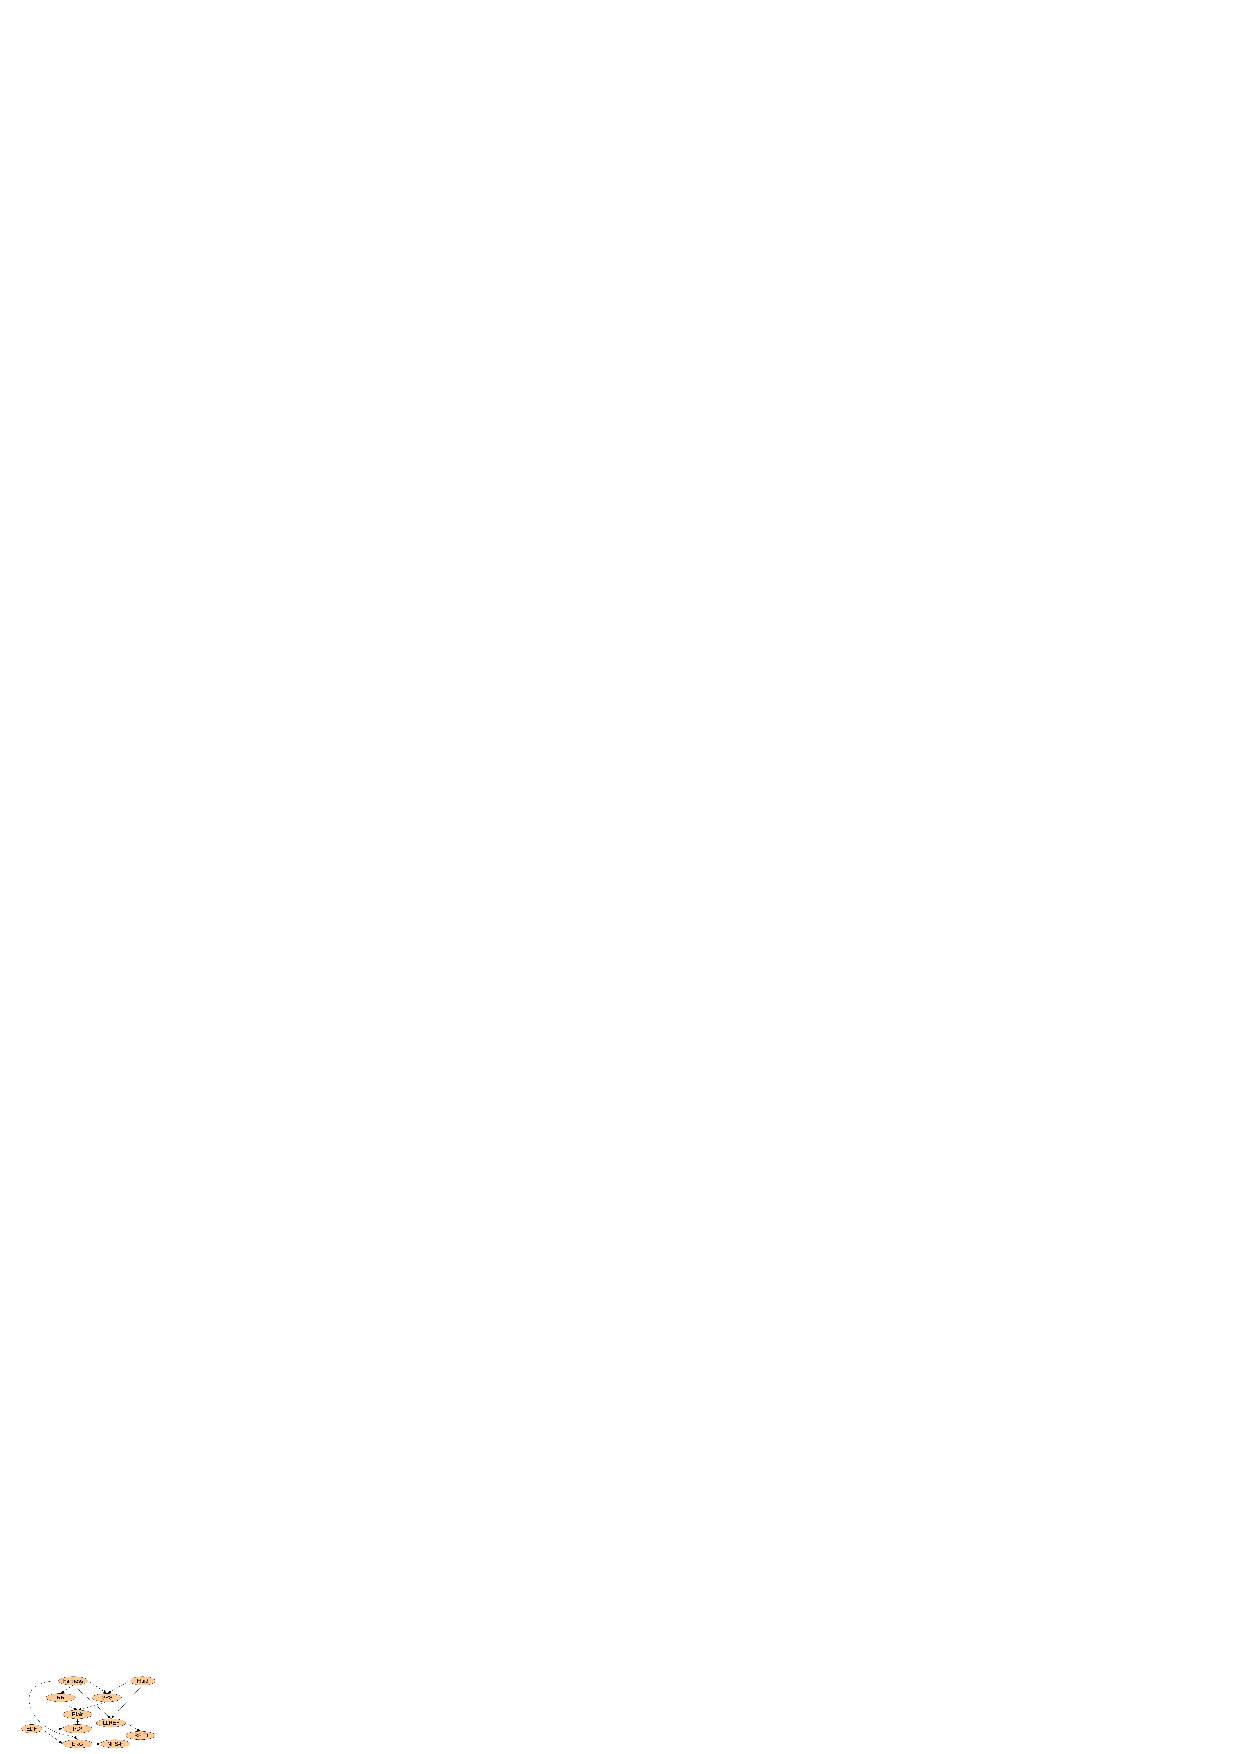
\includegraphics[width=10cm]{img/genealogy_pf}
	\end{figure}
	Ils précisent qu'\textit{EDF} n'est pas concerné par cette classification, mais qu'ayant 
	inspiré certaines approches, il méritait de se trouver sur cette image. 
	Nous invitons le lecteur intéressé par les influences des algorithmes entre eux 
	à prendre connaissance de cet article extrêmement documenté.\medskip
	
	De la lecture des articles, il ressort qu'une partie non négligeable d'entre eux 
	est de parution récente, ce qui montre l'intérêt scientifique actuel pour ce type d'algorithmes. 
	Bien évidemment, les propositions diffèrent par certaines propriétés. Par exemple, 
	\textit{LB-Pfair} est orienté vers les systèmes critiques tolérants aux erreurs. 
	Un enjeu très important de ce grand nombre d'algorithmes est de trouver une méthode qui 
	garantisse l'optimalité pour la classe sporadique, tout en conservant de bonnes performances. 
	
	La préoccupation principale actuelle est de trouver un moyen d'améliorer l'utilisation des processeurs (limitée à 
	50\% pour les algorithmes partitionnés \cite{oh_utilization_1998}), sans détériorer les performances par 
	une explosion du nombre de migrations, comme c'est généralement le cas avec des algorithmes globaux. 
	Dans l'article d'Andersson de 2006 \cite{andersson_multiprocessor_2006}, la limite d'utilisation 
	n'est pas aussi importante qu'avec une approche globale, mais le nombre de préemptions est limité par 
	une constante $k$. En 2006 toujours, Cho et al. \cite{cho_optimal_2006} proposent \textit{LLREF} 
	(largest local remaining execution time), dont l'optimalité est prouvée pour les 
	systèmes périodiques. Ses performances ne sont à ce jour pas bien connues en pratique. 
	La liste proposée ici n'est pas exhaustive, un très grand nombre de propositions existe actuellement. 
	
	\subsection{EDF-k}
	En 2003, Goossens et al. proposent l'algorithme \textit{EDF-k} \cite{goossens_priority-driven_2003}, 
	dont l'idée principale est d'être basé sur la priorité. 
	La définition de \textit{Priority-driven Algorithm} (axé sur les priorités) 
	est donnée par Ha et Liu en 1994 :
	\begin{mydef}
		A Scheduling algorithm is said to be a priority driven scheduling algorithm if and 
		only if it satisfies the condition 
		that for every pair of jobs $J_i$ and $J_j$, if $J_i$ has a higher priority than $J_j$ at 
		some instant in time, then $J_i$ always has higher priority than $J_j$.
	\end{mydef}
	(Un algorithme d'ordonnancement est considéré comme axé sur les priorités si et seulement si il 
	satisfait la condition suivante que pour chaque paire $J_i$ et $J_j$, si $J_i$ a une plus 
	grande priorité que $J_j$ à un instant, $J_i$ a alors toujours une plus grande priorité 
	que $J_j$.)\medskip
	Suivant cette idée, \textit{EDF} est axé sur les priorités, là où \textit{PF} ne l'est pas.\medskip
	
	Reprenant l'idée précédente de \textit{EDF-US} dont certaines tâches étaient de priorité 
	supérieures, et d'autres de priorité simplement assignées par \textit{EDF} \og classique\fg{} , 
	le nombre $k$ représente le nombre stable de tâches ($-1$) concernées par ces priorités 
	supérieures. En d'autres termes, \textit{EDF-k} donne la priorité la plus élevée à 
	$k - 1$ tâches, tandis que les autres sont ordonnancées suivant \textit{EDF}.\medskip
	
	L'article propose une équation dont on dérive la valeur optimale de $k$, et où l'on peut 
	atteindre $m$ le plus petit, cette valeur étant améliorée par rapport à \textit{EDF-US}.\medskip
	
	Une autre approche consiste à considérer la laxité pour modifier \textit{EDF}. 
	Ainsi, l'idée d'\textit{EDZL} (Earliest Deadline until Zero Laxity) \cite{cirinei_edzl_2007} ou encore d'EDCL \cite{kato_real-time_2007}
	(Earliest Deadline Critical Laxity). \medskip
	
	Des travaux récents continuent d'implémenter des versions d'\textit{EDF} avec stratégie 
	globale, par exemple \textit{GEDF} \cite{li_global_2015} \cite{nelissen_geoffrey_efficient_2013}, donnant lieu à \textit{PGEDF}. Cette 
	branche continue donc d'être étudiée et présente des intérêts.
	
	\subsection{U-EDF}
	\textit{U-EDF} est présenté en 2011 par Nelissen et al. \cite{nelissen_reducing_2011}. Il n'est pas \og \textit{P-Fair}\fg{} , et se démarque donc d'une bonne partie des algorithmes 
	par le fait qu'il ne cherche pas à vérifier de condition de \og P-équité\fg{} .
	Il prend en charge les systèmes périodiques à échéances implicites, et est optimal pour cette classe. 
	Tout d'abord, la preuve de son optimalité se limite aux tâches périodiques dont on a dit plus haut qu'elles 
	ne représentaient pas la majorité des classes e tâches des systèmes embarqués. 
	En 2012, la preuve de son optimalité est élargie aux systèmes sporadiques par Nelissen et al. \cite{nelissen_u-edf_2012}. Le principal but de cet algorithme est de 
	réduire le nombre de préemptions, ce qui est un grand inconvénient de l'approche globale. 
	Soit $m$ le nombre de processeurs, notons que dans le cas particulier où $m = 1$, alors 
	U-EDF $\equiv$ EDF. 
	
	\subsection{RUN}
	Reduction to UNiprocessor (\customhighlight{RUN}) est un algorithme présenté par Regnier et al. en 2013 \cite{regnier_multiprocessor_2013}. 
	Cet algorithme est appliqué aux systèmes périodiques préemptifs à tâches indépendantes à 
	échéances implicites. \textit{RUN} -- contrairement aux exemples vus précédemment -- n'applique pas 
	la \textit{P-Fairness}, et parvient à réduire significativement le nombre de préemptions. 
	\textit{RUN} réduit un ensemble de tâches en plus petits ensembles plus facilement ordonnançables 
	en suivant deux opérations :\medskip
	\begin{itemize}
		\item Une opération \og \textit{Dual}\fg{} 
		\item Une opération \og \textit{Pack}\fg{} 
	\end{itemize}
	Un \textit{Dual} se construit par complémentarité avec un \textit{Primal}, dont les règles de constructions sont 
	données dans l'article.
	Un serveur est chargé d'ordonnancer chaque sous-système. Celui-ci fonctionne à l'aide 
	d'\textit{EDF}, dont les avantages nombreux ont déjà été évoqués plus tôt dans ce document. 
	Il n'est pas évident à la lecture de l'article de comprendre en quoi 
	diffère l'approche de \textit{RUN} par rapport à un ordonnanceur 
	partitionné qui donnerait lieu à des systèmes ordonnancés à l'aide d'\textit{EDF}. 
	En réalité, \textit{RUN} n'est pas un algorithme global, mais plutôt 
	semi-partitionné, et la différence tient particulièrement du fait que les systèmes ne sont pas 
	gérés par des processeurs distincts mais par des serveurs.  
	Les auteurs insistent sur les avantages théoriques de \textit{RUN}, qui devraient motiver une implémentation 
	pratique afin de tester ses avantages. Cette implémentation a été faite 
	\cite{compagnin_putting_2014} sur $LITMUS^{RT}$, et dont les résultats demandent à 
	être confirmés mais montrent les bonnes performances sur ce système.\medskip
	
	\textit{RUN} -- malgré son apparition récente -- a déjà des successeurs. \textit{QPS}
	(Quasi Partitioned Scheduling) est un algorithme 
	également semi-partitionné, mais à la différence de \textit{RUN}, il peut ordonnancer les systèmes de tâches indépendantes sporadiques à échéances implicites. 
	Il est décrit dans un article de Massa et al. \cite{massa_outstanding_2014} en 2014. 
	Comme pour \textit{RUN}, \textit{QPS} génère des sous-ensembles de tâches qui seront ordonnancés 
	selon \textit{EDF} par des serveurs. Les auteurs présentent l'avantage d'une approche semi-partitionnée, 
	qui fait un compromis entre les avantages de l'approche partitionnée et ceux de l'approche globale 
	mais \textit{RUN} comporte quant à lui l'inconvénient de ne pas pouvoir s'appliquer aux tâches sporadiques. C'est ce qui explique la nécessité de l'existence de \textit{QPS}.
	L'avantage de \textit{QPS} est de pouvoir adapter sa stratégie en fonction de la
	charge. En effet, durant l'exécution, \textit{QPS} peut s'adapter, passant d'une
	stratégie \textit{globale} à \textit{partitionnée}, ou le contraire. 
	Pour ce faire, \textit{QPS} va diviser les tâches en sous-systèmes, classés différemment selon leur besoin en processeur :\medskip
	\begin{itemize}
		\item \textit{mineur}, si le sous-système a besoin d'un seul processeur
		\item \textit{majeur}, si le sous-système a besoin de plusieurs processeurs
	\end{itemize}
	Par conséquent, si tous les sous-systèmes sont mineurs, \textit{QPS} fonctionne comme 
	\textit{EDF} partitionné. Dans le cas contraire, l'exécution dépendra des besoins 
	des sous-systèmes, et pourra être composé de plusieurs \textit{serveurs QPS} 
	en mode multi-processeur, ou en \textit{EDF} sur simple processeur, cumulant 
	deux modes. \medskip
	Les résultats attendus de \textit{QPS} sont donc très prometteurs, car il permet de 
	conjuguer les avantages des approches partitionnées ainsi que globales.
	
	